
%%% Local Variables: 
%%% mode: latex
%%% TeX-master: t
%%% End: 

\chapter{基于命名数据网络的存储服务}
\label{repo}

\section{命名数据网络存储原型介绍}
在NDN中,缓存结构(CS)直接集成在NDN的架构之中,但CS架构还不能完全满足复杂的内容操作要求:一方面CS只是数据的缓存,数据会被替换掉;另一方面对于数据的插入,删除,访问控制等问题,CS完全没有主动操作接口。NDN网络架构取代当前的IP网络架构的一个主要动机就是,当前网络最主要的流量是数据分发,NDN以数据为中心的拉模式(pull)也非常适合数据分发类的应用。

CS可以将数据直接存储在网络层,而相应数据存储应用也可以将数据存储在网络直接可操作的层面。NDN架构支持网络层次存储的的主要原因为:1.NDN直接以数据本身的名字进行命名。在IP网络中,数据以源地址和目的地址进行命名,数据无法被其他主机重用。虽然有组播的方式,但是对于组播组之外主机还是无法进行重用。2.数据隐私:每一个命名数据都带着签名,数据的非拥有者无法对数据进行篡改。同时数据发布者可以对数据直接进行加密,数据的私密性也可以得到保证。

在NDN中,数据仓库(repository,简称repo)为持久数据存储模型。在NDN中,NDN Repo的概念为被单一组织管理的运行在NDN网络上的数据存储应用。NDN Repo直接运行在NDN网络之上,而不是去修改NDN的底层协议。Repo最主要的作用就是为数据提供持久存储,处理NDN网络转发的数据请求(inerest)。Repo的存储单位为数据对象(data object),数据的管理单位为\textit{data object}的名字前缀。NDN Repo需要遵守NDN Repo协议,该协议定义了操作Repo的基本语义与流程。协议内容基本包括数据的插入,删除以及查询。Repo协议中为数据的访问控制,安全信任提供了框架,但是没有具体规定访问政策与信任模型。同时NDN Repo实现了应用层网络封装的概念。\cite{clark1990architectural}

同NDN直接的数据分发功能相比,NDN Repo还需要支持对于应用的操作功能,需要规范相应的远程操作协议,同当今互联网Web服务类似,需要控制指定名字的服务提供者提供标准的接口与流程协议文档。需要在NDN数据基础上进一步地进行服务抽象。

在CCNx\footnote{CCNx: http://www.ccnx.org/what-is-ccn/}项目中,有类似的CCNr\footnote{Ccnr: https://www.ccnx.org/releases/latest/doc/technical/RepoProtocol.html}项目。而CCN项目与NDN项目都源自与文献\cite{jacobson2009networking}的最初架构设计。虽然CCNr同样提供数据的存储、插入等功能。但是CCNr不支持远程插入数据,不支持删除,没有任何访问控制策略。

\section{命名数据网络存储协议原则}
NDN Repo需要支持数据的远程的插入和删除功能。为了实现这样的功能,需要Repo服务请求者发送“命令”到Repo来实现相应的功能。在这个过程中,Repo需要完成起码三点工作:“命令”可以被转发到指定的Repo,指定的Repo需要有可以被标示的身份以及repo能够验证“命令”发送者的身份以及权限。

NDN Repo协议是一组操作与控制指定Repo的通信协议。在数据传输与Repo控制过程中所涉及到流量控制,访问控制,信任模型等需要NDN Repo在遵守该协议之外去具体定义。在设计NDN Repo协议之前需要解决如下的问题:
\begin{enumerate}
\item \textbf{Repo的存储单位是什么:}NDN Repo的存储单位为数据对象(data object)。一个数据对象不仅仅局限于一个NDN网络数据包,而是被NDN网络上层应用所定义。一个数据对象遵循NDN网络的命名规范,并可以被分段成多个NDN网络包。虽然数据请求者还是可以请求具体的数据段,但是在插入和删除等命令中,数据还是以对象为单位进行操作。
\item \textbf{Repo提供什么功能:}对于一个存储系统来说最基本的功能是\textit{CRUD}。当前Repo提供数据的获取,插入与删除功能。数据插入分为两种,一种是插入指定的数据对象,另一种是使Repo不停地请求指定前缀的数据。
\item \textbf{如何识别指定的Repo:}Repo通过NDN名字前缀来制定,作为interest中名字的前缀来进行转发。
\item \textbf{如何设计Repo命令与响应:}NDN中基本的通信流程为数据请求者发送interest,NDN网络返回命名数据包。因此Repo服务请求信息有两种选择,即封装在interest或者命名数据包中。如果封装在数据包中,则需要服务请求者首先发送一个吸引请求(soliciting interest)使repo能够根据soliciting interest封装的信息去发送服务文档请求interest。另一种模式是将整个服务请求文档封装在interest中,直接发送到指定的Repo。在前一种选择中,soliciting interest还是需要封装一定信息,在通信过程中也造成一定的浪费。本协议设计采取后一种方案。

命令响应为服务请求interest的数据返回包,响应结果文档封装在该数据包的内容中。
\item \textbf{如何制定Repo的安全设计:}在NDN原始架构中,对于数据包的安全性已经得到很大支持。但没有太多对interest安全性的设计支持。但是对于数据的安全性设计可以应用在interest之中,即在interest中加入签名,公钥等信息。Repo可以对interest进行验证,同时可以利用interest中的公钥信息来进行访问控制。
\item \textbf{如何设计Repo服务流程:}为了控制Repo的服务流程,流入数据插入的流程,Repo端的状态需要对服务请求者可见。而对于NDN基础的通信流程,一个interest只能对应的返回一个数据包,只通过单一的服务请求interest服务了解Repo服务状态。在NDN Repo协议设计中,每一个服务相应的有服务状态检查设计。
\end{enumerate}
\subsection{数据获取}
Repo的数据获取采用NDN一般的数据获取方式,即通过返回interest所对应的数据包。在具体的Repo实现中,可以增加数据前缀以及Interest发送者身份的访问控制
\subsection{数据插入}
Repo插入过程起始于请求者发送数据插入命令。与IP网络中推的模式不同,数据源无法直接将数据发送给Repo,需要Repo根据命令interest所封装的参数来发送数据请求interest。可以看到,在本过程中,请求者无法控制Repo从具体哪个主机取得数据,但是数据请求者可以在interest中增加限制条件(seletcor\footnote{Selector:http://named-data.net/doc/ndn-tlv/interest.html\#selectors})来对数据发布者等进行限制。

NDN Repo提供三种基本的插入协议:
\begin{itemize}
\item \textbf{单独插入:}通常用来插入比较小的数据对象,数据通常可以封装在一个最大传输单元(MTU)中。
\item \textbf{选择子插入:}在普通的数据请求interest中,选择子(selector)是用来增加除了数据名字外的限制条件的,比如限制名字的长度等。选择子请求就是要repo在请求数据的过程中加入指定的selector。
\item \textbf{分段插入:}分段插入命令是用来插入比较大的数据对象,即不能完整的封装一个MTU,需要进行分段。Repo通过发送多个interest,interest名字的尾部附加递增的段序号。interest发送的方式由应用自己来定义,可以采用线性方式,也可以采用流水线方式。由于获取数据过程中需要发送大量interest,这个过程中可能会产生网络拥塞。在Repo应用的开发过程中,用户需要自己定义流量控制与拥塞避免的方式。

\end{itemize}

Repo协议同样支持插入状态查询命令。当Repo接收到查询状态命令时,会返回一个状态码来表示执行状态。当该插入过程为分段插入时,Repo会返回当前的插入进度。

在分段插入的过程中,插入命令需要指定数据对象的起始段ID与结束段ID。当插入命令中没有指定结束ID的时候,Repo会一直发送ID号递增的interest。返回的数据中可以附带结束ID字段FinalBlockId\footnote{FinalBlockId:http://named-data.net/doc/ndn-tlv/data.html\#finalblockid}。如果Repo始终无法确定结束端ID到一定时常后,会触发无结束超时(noEndTimeout),此时Repo会停止发送interest。但是,某些情况下,用户想进行实时的数据插入,即刚开始无法确定数据对象的大小,所以需要一种避免noEndTimeout的机制。在Repo协议设计中,可以定期发送插入状态检查命令来noEndTimeout的计时器重新置0,来增加插入的时间。

Repo协议还包括丢包重传机制。当Interest在一定时间内未被响应的时候,repo会重新发送interest。当interest多次重传未被满足时,Repo会停止插入过程。
\subsection{数据删除}
当Repo的存储容量持续膨胀时,或某些数据已经过期、错误时,Repo需要支持删除命令。整个删除过程为,请求者发送删除命令,Repo解析命令并删除相应数据,最后发回给请求者。Repo删除命令分为如下三种。

\begin{itemize}
\item \textbf{单独删除:}单独删除会删除以改名字为前缀的\textbf{所有}数据。
\item \textbf{选择子删除:}要删除的数据对象的选择条件为数据的名字前缀外加选择子,删除所有满足条件的数据对象。与普通意义上的selector不同,普通interest中selector是用来选择满足限制条件的某一个interest。但是在删除协议中,选择子用来选择所有满足条件的数据对象。
\item \textbf{分段删除:}分段删除可以指定所删除数据对象的段范围,即起始段ID与结束段ID之间的数据包
\end{itemize}

综上所述,删除协议是在一定的条件下删除尽可能多的数据,在单独删除中,删除命令会删除指定前缀下的所有数据,这样可以减小删除数据所需要发送的interest的数量。如果要删除某一个数据对象则需要指定某个数据对象的全名并利用选择子指定该对象的数据长度。

在删除过程中依然有删除状态检查命令。由于在删除的过程中,是先发送命令,等数据删除之后才能接收到结果返回,这个过程有可能比较长,而删除请求者一般会分配资源去等待返回结果。通过周期性的发送删除命令可以了解删除进度,请求者可以设定一定的超时时间来中断删除过程并释放资源。

\subsection{前缀插入}
前缀插入是一种特殊的插入方式,该方式是让Repo在一定时间内持续发送同样名字前缀的数据请求。这种方式不仅可以插入已经存在的数据对象,更加适合实时插入新生成的数据。例如在视频通话场景中,需要数据实时地生成。与普通插入相比,普通插入是一个即时的过程,而前缀插入是一个持续的过程。

前缀插入命令需要指定需要插入的数据前缀,选择子,插入过程持续时间,以及无数据返回的超时时间等。为了保证返回的数据不重复,每当数据返回时,Repo需要更新interest的排除选择子(Exclude Selector\footnote{http://named-data.net/doc/ndn-tlv/interest.html\#exclude})。

\section{命名数据网络存储服务协议细节}
NDN repo协议是规定了操纵NDN持久存储的语义以及流程。 NDN repo提供了数据对象获取,插入,删除等功能。 NDN Repo需要遵守NDN Repo协议中的操作流程以及语义,但是并不需要规定特定的存储模式,安全模型,同样也不需要保证对于特定操作一定要返回真实,正确的结果。NDN Repo协议包含以下子协议:

\begin{itemize}
\item \textbf{Repo命令协议}规定了Repo协议中服务请求以及服务响应的格式与语义,同时规定了如何加入安全信息作为Repo安全模型建立的基础
\item \textbf{Repo基础插入协议}规定了如何在Repo插入一个数据包已经数据对象,除了基础的插入协议之外,还有两种特殊的插入协议:前缀插入协议以及TCP后台批量插入协议。
\item \textbf{Repo删除协议}规定了从Repo中删除对象的操作语义与流程
\end{itemize}

\subsection{Repo命令协议}
Repo命令的格式封装遵循NDN signed interest\footnote{Signed interest: http://named-data.net/doc/ndn-cxx/0.3.1/tutorials/signed-interest.html}的格式,格式如下:

\begin{framed}
\begin{scriptsize}
\begin{verbatim}
/<repo-prefix>/<command-verb>/................./.........................................
                              \______  _______/ \__________________  ___________________/
                                     \/                            \/
                             RepoCommandParameter   Signed Interest additional components
\end{verbatim}
\end{scriptsize}
\end{framed}

Repo命令实际上为在NDN名字基础上,通过修改每个名字子单元结构,增加结构化参数得到的。Repo命令interest的名字单元意义如下所示:


\begin{itemize}
\item $\langle repo-prefix\rangle$ 为Repo监听的命令名字前缀
\item $\langle command-verb\rangle$ 为代表Repo具体命令的动词,例如\textit{insert},\textit{delete}等
\item $\langle RepoCommandParameter\rangle$ 为执行特定命令需要的参数。由于Repo命令采用NDN interest进行封装。在现行的NDN协议中,网络数据包用的是TLV(Type Length Value)格式进行封装。该格式可以像xml格式一样迭代的封装子单元。在RepoCommandParameter可以封装多个参数。
\end{itemize}

在Signed Interest additional components采用的是signed interest格式对进行签名。signed interest包含的结构如下所示:
\begin{itemize}
\item $\langle timestamp\rangle$ 为命令的时间戳,为非负整数。时间戳用来防止重复攻击(replay attack)。
\item $\langle random-value\rangle$ 随机值用来确保每一个命令的唯一性。
\item $\langle SignatureInfo\rangle$ 签名信息用来封装签名类型,采用算法,签名证书位置(KeyLocator)等信息.
\item $\langle SignatureValue\rangle$用来封装实际签名值。
\end{itemize}

对于前缀为/ucla/cs/repo的NDN repo服务,命令如下所示
\begin{framed}
\begin{tiny}
\begin{verbatim}
/ucla/cs/repo/<command verb>/<RepoCommandParameter>/<timestamp>/<random-value>/<SignatureInfo>/<SignatureValue>
\end{verbatim}
\end{tiny}
\end{framed}

\subsubsection{RepoCommandParameter}
对于TLV文档,有其一套定义文档。RepoCommandParameter的定义如下:
\begin{framed}
\begin{footnotesize}
\begin{verbatim}
RepoCommandParameter ::= REPOCOMMANDPARAMETER-TYPE TLV-LENGTH
                           Name?
                           Selectors?
                           StartBlockId?
                           EndBlockId?
                           ProcessId?
                           MaxInterestNum?
                           WatchTimeout?
                           WatchStatus?
                           InterestLifetime?



Name                  ::= NAME-TYPE TLV-LENGTH NameComponent*
NameComponent         ::= NAME-COMPONENT-TYPE TLV-LENGTH BYTE+

Selectors             ::= SELECTORS-TYPE TLV-LENGTH
                           MinSuffixComponents?
                           MaxSuffixComponents?
                           PublisherPublicKeyLocator?
                           Exclude?
                           ChildSelector?

MinSuffixComponents   ::= MIN-SUFFIX-COMPONENTS-TYPE TLV-LENGTH
                           nonNegativeInteger

MaxSuffixComponents   ::= MAX-SUFFIX-COMPONENTS-TYPE TLV-LENGTH
                           nonNegativeInteger

PublisherPublicKeyLocator ::= KeyLocator

Exclude               ::= EXCLUDE-TYPE TLV-LENGTH Any? (NameComponent (Any)?)+
Any                   ::= ANY-TYPE TLV-LENGTH(=0)

ChildSelector         ::= CHILD-SELECTOR-TYPE TLV-LENGTH
                           nonNegativeInteger

StartBlockId          ::= STARTBLOCKID-TYPE TLV-LENGTH
                           nonNegativeInteger

EndBlockId            ::= ENDBLOCKID-TYPE TLV-LENGTH
                           nonNegativeInteger

ProcessId             ::= PROCESSID-TYPE TLV-LENGTH
                           nonNegativeInteger

MaxInterestNum        ::= MAX-INTEREST-NUM-TYPE TLV-LENGTH
                           nonNegativeInteger

WatchTimeout          ::= WATCH-TIMEOUT-TYPE TLV-LENGTH
                           nonNegativeInteger

WatchStatus           ::= WATCH-STATUS-TYPE TLV-LENGTH
                           nonNegativeInteger

InterestLifetime      ::= INTEREST-LIFETIME-TYPE TLV-LENGTH
                           nonNegativeInteger
\end{verbatim}
\end{footnotesize}
\end{framed}

上述文档描述了Repo命令参数的结构以第一行为例,其中RepoCommandParameter为参数名,REPOCOMMANDPARAMETER-TYPE为参数类型,在TLV中通过预先定义的数字来表示。Name为后面TLV子结构的名字。在Name中,可以看到由多个NameComponent组成。在NameComponent中,其实际类型为BYTE+。

\textbf{Repo Command Selectors}

Repo命令支持部分的interest选择子(selector)。选择子的作用是在interest的名字前缀会对应多个数据时所增加的限制条件。NDN interest selector和RepoCommandParameter在意义上有所不同。NDN interest selector可以用来直接选择数据包。而repo选择子在不同的命令下,含义有所不同。

在插入命令中,基本流程为插入请求端发送插入命令,repo解析命令中的参数,并根据参数发送一般的NDN interest来获取数据。在RepoCommandParameter中的selector则会被直接添加到repo发送的interest中作为数据选择限制条件。在删除命令中,选择子被用来直接选择要删除的数据。同一般selector不同的是,普通选择子选择满足条件的一个数据包,而删除命令中的选择子会选择满足条件的所有数据包。

Repo Command支持部分选择子,包括 MinSuffixComponents,MaxSuffixComponents,PublisherPublicKeyLocator和Exclude. ChildSelector 选择子只是在插入命令中支持,在删除命令中不支持。如果命令中包含不支持的选择子,则repo会忽略这些不支持的选择子。选择子的格式如下所示:
\begin{framed}
\begin{footnotesize}
\begin{verbatim}
Selectors             ::= SELECTORS-TYPE TLV-LENGTH
                           MinSuffixComponents?
                           MaxSuffixComponents?
                           PublisherPublicKeyLocator?
                           Exclude?
                           ChildSelector?

MinSuffixComponents   ::= MIN-SUFFIX-COMPONENTS-TYPE TLV-LENGTH
                           nonNegativeInteger

MaxSuffixComponents   ::= MAX-SUFFIX-COMPONENTS-TYPE TLV-LENGTH
                           nonNegativeInteger

PublisherPublicKeyLocator ::= KeyLocator

Exclude               ::= EXCLUDE-TYPE TLV-LENGTH Any? (NameComponent (Any)?)+
Any                   ::= ANY-TYPE TLV-LENGTH(=0)

ChildSelector         ::= CHILD-SELECTOR-TYPE TLV-LENGTH
                           nonNegativeInteger
\end{verbatim}
\end{footnotesize}
\end{framed}

\textbf{StartBlockId, EndBlockId}

StartBlockId与EndBlockId表示要插入和删除数据对象的分段的范围。在发送命令中,两者都可以不存在。StartBlockId的默认值为0。当EndBlockId不存在是,在插入命令中,Repo会不断发送更大的数据分段请求,

\textbf{Selector与StartBlockId和EndBlockId冲突}

在插入命令中如果采用Id范围的话,则需要插入的数据名字为数据对象完整的名字。而Selector则是以改名字为前缀选择一个数据对象。当Selector和数据段范围同时存在的时候,Repo则忽略该命令并返回表示格式错误的状态码(405)。

\textbf{ProcessId}

为了使repo能够处理多个插入或删除过程,通过ProcessId用来区分不同的过程。

\textbf{InterestLifetime}

InterestLifetime指的是从Interest发送到data接收的最大延迟时间。在插入命令中,InterestLifetime会被添加在数据获取interest中。在删除命令中,InterestLifetime指的是删除命令从发送到最后得到结果的最大等待时间。

\textbf{MaxInterestNum}

MaxInterestNum为前缀插入命令的参数,表示的是Repo对于同一前缀最多可以发送的interest数目。

\textbf{WatchTimeout}

WatchTimeout为前缀插入命令的参数,表示的是Repo对于同一前缀的前缀插入进程最长的保持时间,超过该时间,Repo会结束前缀插入的过程。

\textbf{WatchStatus}

WatchStatus为前缀插入命令的参数,该参数为客户端在Repo前缀插入过程中的主动控制参数。当WatchStatus为false的时候,会主动关闭Repo前缀插入的过程。

\subsubsection{Repo Command Response}
Repo Command Response是repo对于相对应的repo命令的返回数据包。在Repo Command Response中通过状态码statuscode来表示所对应的repo命令进程的运行状态。在该命令返回包中,封装了一些关于repo运行状态的信息,通过TLV子结构RepoCommandResponse封装在数据包的内容部分之中。RepoCommandResponse的文档描述结构如下所示:

\begin{framed}
\begin{footnotesize}
\begin{verbatim}
RepoCommandResponse   ::= INSERTSTATUS-TYPE TLV-LENGTH
                           ProcessId?
                           StatusCode
                           StartBlockId?
                           EndBlockId?
                           InsertNum?
                           DeleteNum?

ProcessId            ::= PROCESSID-TYPE TLV-LENGTH
                            nonNegativeInteger 

StatusCode            ::= STATUSCODE-TYPE TLV-LENGTH
                            nonNegativeInteger    

StartBlockId          ::= STARTBLOCKID-TYPE TLV-LENGTH
                            nonNegativeInteger

EndBlockId            ::= ENDBLOCKID-TYPE TLV-LENGTH
                            nonNegativeInteger

InsertNum             ::= INSERTNUM-TYPE TLV-LENGTH
                            nonNegativeInteger

DeleteNum             ::= DELETENUM-TYPE TLV-LENGTH
                            nonNegativeInteger
\end{verbatim}
\end{footnotesize}
\end{framed}

\textbf{Name}

代表所对应的Repo命令中repocommandparameter的名字部分,指的是正在操纵的数据对象的名字前缀。

\textbf{ProcessId}

是由Repo产生的一个随机数字,用来指定其所对应的Repo命令的执行进程序列。在后续客户端与Repo对该进程的交互中,需要在命令或者返回网络包中添加该进程序列号以指明对应执行进程。

\textbf{StatusCode}

StatusCode参考HTTP的状态码,通过一个数字来表示对应Repo执行进程的运行状态。

\textbf{StartBlockId, EndBlockId}

StartBlockId和EndBlockId与RepoCommandParameter中的相同。如果命令中,两个参数都是缺失的,Repo将会将利用目前所知的信息为这两个参数赋值。当StartBlockId缺失的时候,repo会将该值置0。如果EndBlockId确实的时候,repo会将该值设置为无穷大。在插入过程中,EndBlockId还会随着得到数据包中的finalBlockId进行更新。

\textbf{InsertNum, DeleteNum}
InsertNum和DeleteNum表示其所对应的命令插入和删除执行过程中,在该时刻总共插入和删除了多少个数据包。

\subsubsection{Repo TLV类型封装序号}
在TLV格式封装中,对于TLV结构类型的名字,在实际编码数字中用对应的数字进行表示。对应的数字编码如表\ref{tab:tlv-encoding}所示:

\begin{table}[h]
\centering
\caption{TLV Encoding Number}
\label{tab:tlv-encoding}
\begin{tabular}{|l|l|}
\hline
\textbf{Type} & \textbf{Number} \\ \hline
RepoCommandParameter & 201 \\ \hline
StartBlockId & 204 \\ \hline
EndBlockId & 205 \\ \hline
ProcessId & 206 \\ \hline
RepoCommandResponse & 207 \\ \hline
StatusCode & 208 \\ \hline
InsertNum & 209 \\ \hline
DeleteNum & 210 \\ \hline
MaxInterestNum & 211 \\ \hline
WatchTimeout & 212 \\ \hline
WatchStatus & 213 \\ \hline
InterestLifetime & 214 \\ \hline
\end{tabular}
\end{table}

\subsubsection{Repo信任模型}
Repo的信任模型依赖于Repo服务的实施者的具体设计,例如采用PKI架构。 Repo可以采用各种具体设计的验证策略,数据消费者可以自己定义其信任锚点(trust anchor)。但Repo协议中不会定义具体的安全设计,只是提供了建立安全策略与信任模型的基本工具singed interest。NDN信任管理可以具体参见NDN FAQ\footnote{NDN FAQ: http://named-data.net/project/faq/}

\subsection{Repo基础插入协议}
基础repo插入协议利用Repo命令。Repo插入命令触发指定repo获取并存储相应的数据对象。该命令为signed interest,除了验证信任之外,可以通过身份来进行访问控制。当interest可以被验证但是数据对象不存在时,repo会应答表示OK的状态码,并开始发送interest去获取数据对象。

基础插入协议同样支持数据对象分段插入。分段信息定义在RepoCommandParameter中。

\subsubsection{基础插入命令}

\textbf{插入数据}

Command Verb: insert

插入命令的语义遵循repo命令格式。当$\langle repo prefix\rangle$为 /ucla/cs/repo,插入命令如下所示:

\begin{framed}
\begin{scriptsize}
\begin{verbatim}
/ucla/cs/repo/insert/<RepoCommandParameter>/<timestamp>/<random-value>/<SignatureInfo>/<SignatureValue>
\end{verbatim}
\end{scriptsize}
\end{framed}

\textbf{插入状态检查}

Command Verb: insert check

在插入过程中,请求者可以通过发送状态检查命令去查看插入过程的运行状态。 插入状态检查命令同样是signed interest。状态检查的命令示例如下所示:

\begin{framed}
\begin{tiny}
\begin{verbatim}
/ucla/cs/repo/insert check/<RepoCommandParameter>/<timestamp>/<random-value>/<SignatureInfo>/<SignatureValue>
\end{verbatim}
\end{tiny}
\end{framed}

\textbf{插入类型}

如前面协议原则介绍所属,基础插入协议共支持三种插入类型,包括单数据包插入,分段插入以及选择子插入

\subsubsection{格式}
\textbf{RepoCommandParameter}

基础插入命令以及插入状态检查命令中参数RepoCommandParameter遵循repo command协议。其中插入命令使用包括Name,Selectors,StartBlockId和EndBlockId。状态检查命令使用Name和ProcessId。

在插入命令中,名字代表要插入数据对象的名字前缀或完整的名字。如果选择子Selectors被设置的话,repo获取数据的interest中需要附加该选择子。如果StartBlockId或EndBlockId被设置的话,则证明该插入过程为分段插入,repo获取数据对象StartBlockId与EndBlockId之间的分段。因为Selectors中Name的含义为名字前缀,但是在分段插入中,name代表的数据的完整的名字。所以当StartBlockId或EndBlockId与Selector同时被设置时,repo会忽略该命令并返回格式错误信息(405)。

在插入状态检查命令中,名字代表要检查插入状态的命令前缀。ProcessId是通过最开始插入命令所对应的响应包中的ProcessId来设置的。

\textbf{Insertion status response}

插入状态数据对象可以是数据插入或者状态检查命令的数据返回包,并遵循Repo命令返回(epo command response)格式。

StatusCode表明对应的插入状态。InsertNum表示到目前为止已经有多少需要插入的数据对象所对应的数据包插入到repo之中。StartBlockId和EndBlockId表示到目前为止repo所能确定的插入数据段的插入范围。ProcessId在插入命令命令接收并在插入过程开始之前生成的随机数,用来表示插入过程。

在插入命令的响应请求中,Name,ProcessId,StartBlockId和EndBlockId,ProcessId会被设置。当插入命令的EndBlockId为空时,响应数据包的EndBlockId也会为空。

在状态检查命令的响应数据包中,Name,ProcessId,StartBlockId和EndBlockId,ProcessId会被设置。当插入命令的EndBlockId为空时,相应数据包会一直为空,直到获得的数据包中包含FinalBlockId字段。EndBlockId会被FinalBlockId更新。当出现更小的FinalBlockId时,EndBlockId会继续被更新。

插入命令中StatusCode的定义如表\ref{ins-statusCode}所示:

\begin{table}[h]
\centering
\caption{StatusCode对应定义}
\label{tab:ins-statusCode}
\begin{tabular}{|l|l|}
\hline
\textbf{StatusCode} & \textbf{Description} \\ \hline
100 & The command is OK. can start to fetch the data \\ \hline
200 & All the data has been inserted \\ \hline
300 & This insertion is in progress \\ \hline
401 & This insertion command or insertion check command is invalidated \\ \hline
402 & Selectors and BlockId both present \\ \hline
403 & Malformed Command \\ \hline
404 & No such this insertion is in progress \\ \hline
405 & EndBlockId Missing Timeout \\ \hline
\end{tabular}
\end{table}

\textbf{EndBlockId Missing Timeout}

EndBlockId Missing Timeout指的是当分段插入命令参数中EndBlockId也就是最后一个字段的范围没有设置的时候,并且在Repo获取的data包中也长时间没有FinalBlockId,导致Repo长时间无法确定该确定最后一个数据段号是多少的现象。在Repo插入协议中,当该现象达到一定数值即EndBlockId Missing Timeout这个值的时候,repo便会停止数据获取的过程。在Repo插入过程中,有一种情景就是始终无法确定数据对象最后的字段号。为了维持插入过程,repo协议设计了对于某过程,可以根据该过程的进程号发送相应的查询协议,一次可以重新将EndBlockId Missing Timeout置零。

\subsubsection{协议流程}

\textbf{数据插入协议流程}

\begin{enumerate}[step 1.]
\item Repo开始验证命令。如果验证过程没有马上失败,则跳到step 3。
\item 发送代表验证失败的命令请求返回包,停止协议过程。 (StatusCode: 401)
\item 如果参数中StartBlockId和EndBlockId都不存在,则跳到第7步。
\item 如果StartBlockId或EndBlockId其中至少一个出现,同时参数中出现selectors,则返回代表格式错误的数据返回,同时停止Repo插入过程。(StatusCode: 402)
\item 如果StartBlockId和EndBlockId同时出现,并且StartBlockId小于等于EndBlockId,跳到step 7。
\item 发送代表格式错误的数据返回,并终止插入过程。(StatusCode: 403)
\item 等待验证过程结束
\item 如果验证出现错误,则跳到step 2。(StatusCode: 401)
\item 发送代表插入过程开始的数据返回。(StatusCode: 200)
\item 如果StartBlockId和EndBlockId都不存在,则跳到step 16。
\item 发送含有参数中Name和selectors的interest来获取数据。
\item 等待获取过程结束
\item 如果获取过程失败,则跳到step 27。
\item 存储获得的数据包
\item 停止插入过程,插入过程结束
\item 如果StartBlockId,则本进程StartBlockId为0。如果EndBlockId缺失,则进程EndBlockId缺失直到返回数据包包含FinalBlockId,启动EndBlockId Missing Timeout计时器。
\item 将StartBlockId附在Name之后
\item 开始发送包含Name的interest
\item 等待获取过程结束
\item 如果获取过程失败,则跳到step 26
\item 存储获得的数据包
\item 如果获得的数据包包含FinalBlockId,并且FinalBlockId小于当前EndBlockId或者EndBlockId缺失,则将EndBlockId置为FinalBlockId。
\item 如果Name最后一个部分即代表数据段号的部分大于等于EndBlockId,则停止数据获取过程,插入过程结束。
\item 增加Name数据段号1
\item 跳到step 17
\item 再获取该名字数据两次,如果两次都失败则停止插入过程。如果成功,跳到step 21
\item 再获取该名字数据两次,如果两次都失败则停止插入过程。如果成功,跳到step 24
\end{enumerate}
当EndBlockId Missing Timeout计时器启动之后,repo会监视step 17~26。如果超时发生,Repo会停止插入过程。在监视过程中,如果接收到该过程的查询命令,则将计时器重新置零。

\textbf{数据插入状态检查协议流程}
\begin{enumerate}[step 1.]
\item 验证命令,如果成功则跳到step 2,否则跳到step 3
\item 发送代表验证失败的数据返回包,并停止检查过程。(StatusCode: 401)
\item 开始利用进程号以及数据的名字查询插入过程。如果查询成功,则跳到step 5,否则跳到step 4
\item 返回代表查询失败的数据包。(StatusCode: 404)
\item 查询该插入状态,并返回该状态。如果EndBlockId Missing Timeout计时器正在运行,则将该计时器置零
\end{enumerate}

\subsubsection{协议流程图}
基本插入及插入状态查询协议流程如下所示:

\begin{figure}[H]
\begin{framed}
\begin{scriptsize}
\begin{verbatim}
Requester                     Repo                          Data producer
    |                           |                                 |
    |                           |                                 |
  +---+  Insert command       +---+                               |
  |   | --------------------> |   |                               |
  +---+                       |   |                               |
    |                         |   |                               |
  +---+   Confirm start       |   |                               |
  |   | <==================== |   |                               |
  +---+   Reject command      +---+                               |
    |     (with status code)    |                                 |
    |                         +---+     Interest for Data       +---+
    |                         |   | --------------------------> |   |
    |                         +---+                             |   |
    |                           |                               |   |
    |                         +---+       Data segment          |   |
    |                         |   | <========================== |   |
    |                         +---+                             +---+
    |                           |                                 |
    |                           ~                                 ~
    |                           ~                                 ~
    |                           |                                 |
    |                         +---+     Interest for Data       +---+
    |                         |   | --------------------------> |   |
    |                         +---+                             |   |
    |                           |                               |   |
    |                         +---+       Data segment          |   |
    |                         |   | <========================== |   |
    |                         +---+                             +---+
    |                           |                                 |
    |                           |                                 |
    |                           ~                                 ~
    |                           ~                                 ~
    |                           |                                 |
    |                           |                                 |
    |                           |                                 |
  +---+   Status interest     +---+                               |
  |   | --------------------> |   |                               |
  +---+                       |   |                               |
    |                         |   |                               |
  +---+    Status response    |   |                               |
  |   | <==================== |   |                               |
  +---+                       +---+                               |
    |                           |                                 |
    |                           |                                 |
\end{verbatim}
\end{scriptsize}
\end{framed}
\end{figure}

\subsection{Repo删除协议}
Repo删除协议命令格式遵循Repo Command协议。

Repo删除协议支持删除单个对象,同时也支持删除特定名字前缀下面的所有对象。选择子在删除协议中是用来选择多个对象的。在这里,选择子selectors的意义与一般的选择子含义不同。一般选择子含义是选择满足选择子所规定的限制条件中的一个数据对象,而在删除协议中选择子选择的是满足其规定限制条件的所有数据对象。此外删除协议还支持数据对象分段删除,即删除被分段数据对象一定范围的数据包。

\subsubsection{基本操作}
\textbf{删除命令}

Command verb: \textbf{delete}

删除命令遵循Repo Command协议。删除协议支持如协议设计所示支持三种删除包括单独数据对象删除,同前缀数据对象删除以及分段数据对象删除。

删除命令格式例子如下所示:

\begin{framed}
\begin{scriptsize}
\begin{verbatim}
/ucla/cs/repo/delete/<RepoCommandParameter>/<timestamp>/<random-value>/<SignatureInfo>/<SignatureValue>
\end{verbatim}
\end{scriptsize}
\end{framed}

\textbf{删除状态检查}

Command verb: \textbf{delete check}

删除状态检查与插入状态检查相似,同样可以查询某一删除进程的数据删除状态。

删除命令格式如下所示:

\begin{framed}
\begin{scriptsize}
\begin{verbatim}
/ucla/cs/repo/delete check/<RepoCommandParameter>/<timestamp>/<random-value>/<SignatureInfo>/<SignatureValue>
\end{verbatim}
\end{scriptsize}
\end{framed}

\subsubsection{格式}
\textbf{Deletion Command RepoCommandParameter}

删除命令参数包括Name,Selector,StartBlockId,EndBlockId,ProcessId。

Name为需要删除的数据对象名字前缀。

Selector用来选择任意满足条件的数据对象。在删除命令中不支持ChildSelector选择子。

StartBlockId和EndBlockId用来删除分段的数据对象。Repo会删除StartBlockId和EndBlockId之间的数据段。

ProcessId是客户端生成的用来区分不同删除过程的随机数。Repo会将该ProcessId作为进程号与其它进程进行区分。

\textbf{Deletion status check RepoCommandParameter}

Name和ProcessId用来选定特定的删除过程。如果Repo可以通过Name和ProcessId确定该进程,则返回该删除进程状态。否则则返回查询失败。

\textbf{Deletion Check Command Selectors}

在删除状态查询命令中,不支持选择子。如果命令中包含选择子,则repo返回查询失败数据包。

\textbf{Deletion status response}

Deletion status response可以作为删除命令以及删除状态查询命令的数据返回包。

在deletion status response中,数据内容中包括Name,StatusCode,Selector,StartBlockId,EndBlockId,ProcessId,DeletenNum。其中Name,ProcessId,Selector与删除命令中的含义相同。StatusCode利用特定数字代表删除状态。DeleteNum代表有多少数据包已经被删除。

删除StatusCode定义如下所示:

\begin{table}[h]
\centering
\caption{StatusCode对应定义}
\label{tab:del-statusCode}
\begin{tabular}{|l|l|}
\hline
\textbf{StatusCode} & \textbf{Description} \\ \hline
200 & All the data has been deleted \\ \hline
300 & This deletion is in progress \\ \hline
401 & This deletion or deletion check is invalidated \\ \hline
402 & Selectors and BlockId both present \\ \hline
403 & Malformed Command \\ \hline
404 & No such this deletion is in progress \\ \hline
\end{tabular}
\end{table}

\subsubsection{协议流程}
Repo删除协议流程如下所示:
\begin{enumerate}[step 1.]
\item 开始验证删除命令,如果验证失败,则跳到step 3
\item 发送代表验证失败的命令请求应答,停止协议流程。(StatusCode: 401)
\item 查看是否有相同RepoCommandParameter的删除过程存在,如果存在,则等待删除过程结束
\item 如果StartBlockId或EndBlockId和selectors同时存在,则返回代表格式错误的返回值。(StatusCode: 402)
\item 如果selectors,则跳到step 8
\item 查看是否StartBlockId或EndBlockId存在。如果都存在,查看是否StartBlockId小于等于EndBlockId。如果是,则返回代表格式错误的返回。 (StatusCode: 403) 否则跳到step 9
\item 如果StartBlockId,EndBlockId和selectors都不存在,则跳到step 10。
\item 如果删除满足名字前缀与选择子规定条件的所有数据包,跳到step 11
\item 删除StartBlockId和EndBlockId之间的所有数据包。如果StartBlockId缺失,则删除StartBlockId为0。如果EndBlockId缺失,则删除到最后一个数据段的数据包
\item 如果发送命令的lifetime没有超时,则返回代表删除结束的数据包。如果超时,则在一定时间内等待相同名字以及删除参数的命令。删除过程结束。(StatusCode: 200)
\end{enumerate}

Repo删除状态检查协议的流程为:
\begin{enumerate}[step 1.]
\item 验证删除状态检查命令你敢
\item 如果验证失败则返回代表验证失败的数据包,停止检查流程。(StatusCode: 401)
\item 通过ProcessId与名字前缀查询删除过程状态。如果没有改进程,跳到step 4,否则跳到step 5
\item 返回代表查询失败的数据包。 (StatusCode: 404)
\item 返回代表查询成功的数据包。 (StatusCode: 300)
\end{enumerate}

\subsubsection{协议流程图}
删除及删除状态查询协议流程如下所示:

\begin{figure}[H]
\begin{framed}
\begin{scriptsize}
\begin{verbatim}
Requester                     Repo 
    |                           |                                 
    |                           |                                 
  +---+  Delete command       +---+                               
  |   | --------------------> |   |                               
  +---+                       +---+                               
    |                           |                                 
    |                           |                                 
    |                           |                                 
  +---+   Status interest     +---+                               
  |   | --------------------> |   |                               
  +---+                       |   |                               
    |                         |   |                               
  +---+    Status response    |   |                               
  |   | <==================== |   |                               
  +---+                       +---+                               
    |                           |                                 
    |                           |                                 
    |                           |                                 
  +---+   Confirm Deletion    +---+                               
  |   | <==================== |   |                               
  +---+   Reject command      +---+                               
    |     (with status code)    |    
    |                           |
\end{verbatim}
\end{scriptsize}
\end{framed}
\end{figure}

\subsection{Repo前缀插入协议}
前缀插入是一种特殊的Repo数据插入协议。在该协议中,Repo持续发送相同名字前缀的interest。当repo接收到数据包时,repo会更新exclude选择子,从而可以不再接收该名字的数据包,使获得的数据包不重复。Repo会在以下情况,停止前缀插入过程:Repo发送Interest到一定数量或一定时间;interest发送失败到一定数量;Repo接收到前缀插入停止请求。

\subsubsection{基本操作}
\textbf{前缀插入开始命令}

Command Verb: \textbf{watch start}

前缀插入开始命令的格式参照Repo Command协议。 前缀插入命令例子如下:

\begin{framed}
\begin{scriptsize}
\begin{verbatim}
/ucla/cs/repo/watch start/<RepoCommandParameter>/<timestamp>/<random-value>/<SignatureInfo>/<SignatureValue>
\end{verbatim}
\end{scriptsize}
\end{framed}

Watch start命令使用一下参数:

\begin{itemize}
\item Name:为前缀插入发送interest用的前缀,在这个前缀下的数据包会被不断地插入repo之中
\item InterestLifetime:为repo发送的interest与数据最大的延迟时间。当interest超时,则repo会重新发送相同的interest。如果repo在InterestLifetime的时间内接收到数据,则repo发送Interest的selectors的exclude选择子会进行更新,接收到数据的名字会被添加进exclude选择子。repo之后会发送更新过的的interest来获取数据。
\item MaxInterestNum代表repo最多可以发送interest的数量。当发送的Interest到达这个数量时,repo会停止watch prefix过程。如果在命令中没有指定MaxInterestNum,则代表MaxInterestNum为无穷大。
\item WatchTimeout代表watch prefix过程最大的持续时间。当repo发送前缀插入的过程超过了这个时间,如果WatchTimeout没有在命令中指定,则WatchTimeout默认值为无穷大。
\end{itemize}

\textbf{前缀插入状态检查命令}

Command Verb:\textbf{watch check}

watch check用来查询前缀插入的执行状态,遵循repo command协议。watch check命令格式例子如下所示:

\begin{framed}
\begin{scriptsize}
\begin{verbatim}
/ucla/cs/repo/watch check/<RepoCommandParameter>/<timestamp>/<random-value>/<SignatureInfo>/<SignatureValue>
\end{verbatim}
\end{scriptsize}
\end{framed}

watch prefix采用Name和ProcessId作为参数条件用来匹配对应的Watch Prefix过程

\textbf{前缀插入停止命令}

Command Verb:\textbf{watch stop}

在repo前缀插入过程中,当其接到前缀插入停止命令,对应的前缀插入过程会停止。watch stop命令遵循Repo Command协议,其格式例子如下所示:

\begin{framed}
\begin{scriptsize}
\begin{verbatim}
/ucla/cs/repo/watch stop/<RepoCommandParameter>/<timestamp>/<random-value>/<SignatureInfo>/<SignatureValue>
\end{verbatim}
\end{scriptsize}
\end{framed}

前缀插入停止命令采用Name和ProcessId作为参数条件用来匹配对应的Watch Prefix过程。

\subsubsection{RepoCommandResponse}
前缀插入过程的RepoCommandResponse可以同时作为前缀插入命令与前缀插入状态检查命令的数据返回。RepoCommandResponse主要包含两个参数:InsertNumber代表有多少数据包已经被插入到repo中;StatusCode用数字代表前缀插入过程运行的状态。

前缀插入的StatusCode定义如下所示:

\begin{table}[h]
\centering
\caption{StatusCode对应定义}
\label{tab:watch-statusCode}
\begin{tabular}{|l|l|}
\hline
\textbf{StatusCode} & \textbf{Description} \\ \hline
100 & The command is OK. Start to watch the prefix \\ \hline
101 & Watched Prefix Insertion is stop \\ \hline
300 & This watched prefix Insertion is in progress \\ \hline
401 & This watch command or watchCheck command is invalidated \\ \hline
402 & BlockId present. BlockId is not supported in this protocol \\ \hline
403 & Malformed Command \\ \hline
404 & No such this process is in progress \\ \hline
\end{tabular}
\end{table}

\subsubsection{前缀插入协议流程}
\textbf{前缀插入开始协议流程}

\begin{enumerate}[step 1.]
\item 开始验证watch start命令。如果验证成功,跳到step 3,否者跳到step 2
\item 返回代表验证不成功的数据返回。结束前缀插入过程。 (StatusCode: 401)
\item 检验前缀插入命令参数,如果无法成功提取,则返回代表格式错误的数据返回,停止前缀插入过程。(StatusCode: 403)
\item 如果参数中包含BlockId,则代表返回格式不支持的数据返回,结束前缀插入过程。(StatusCode: 402) 
\item 利用提取出来的参数构建interest,并将selector设置为Rightmost Child Selector。
\item 发送Interest并启动watchtime计时器以及发送Interest的计数器并将计数器置1
\item 如果接收到数据,跳到step 8,如果interest超时,则跳到step 17
\item 如果数据可以被验证,则跳到step 9,否则跳到step 15.
\item 检查是否前缀插入过程还在执行,如果停止执行,则流程结束。
\item 检查前缀插入整个过程是否超时或者发送interest数据达到规定上限,如果是跳到step 11,否则跳到step 12
\item 清空流程变量(sent interest数量,watch timeout, interest lifetime),并停止插入流程
\item 将数据存入repo之中
\item 更新selectors,将接受数据包名字加入exclude选择子中,并构造新的interest
\item 发送新的interest并将计数器加1,跳到step 7.
\item 重复step 9到step 11,并跳到step 12
\item 更新选择子并跳到step 14
\item 重复step 9到step 11,并跳到step 12
\item 发送新的interest并将计数器加1,跳到step 7.
\end{enumerate}

\textbf{前缀插入状态检查协议流程}

\begin{enumerate}[step 1.]
\item 开始验证命令。如果验证成功跳到step 3,否则跳到step 2
\item 返回代表验证不成功的数据返回。结束状态检查流程那个。 (StatusCode: 401)
\item 检验前缀插入状态检查命令参数,如果无法成功提取,则返回代表格式错误的数据返回,停止前缀插入过程。(StatusCode: 403)
\item 检查该进程是否存在,如果存在,跳到step 5,否则发送代表查询失败的数据返回。(StatusCode: 404)
\item 利用processId去查找数据返回,并返回前缀插入运行状态
\end{enumerate}

\textbf{前缀插入停止协议流程}

\begin{enumerate}[step 1.]
\item 验证停止命令。如果验证成功跳到step 3,否则跳到step 2
\item 发送达标验证失败的数据返回,停止前缀插入的关闭流程。 (StatusCode: 401)
\item 提取前缀插入停止命令参数,如果无法提取参数,则返回代表格式错误的数据返回。(StatusCode: 403)
\item 停止前缀插入流程并返回代表停止成功的数据返回。 (StatusCode: 101)
\end{enumerate}


\section{命名数据网络存储服务开发及实验评估}
基于NDN Repo协议,作者开发了repo-ng(NDN repo of next generation)作为协议的原型实现。repo-ng的设计原则是希望能做到跨平台,降低对系统的特殊依赖,并且尽量轻量级。repo-ng采用ndn-cxx作为NDN协议底层开发库,利用sqlite3\footnote{SQLite3:https://sqlite.org/about.html}数据库作为数据对象底层存储。

\subsection{存储设计}
Repo后台存储包括索引和存储两个模块。索引用来存储数据名字的有序数据结构,存储模块用来存储完整的数据包及数据包其他信息。在repo-ng实现中,后台存储采用sqlite3数据库。选择sqlite3数据库是因为sqlite3的快平台性,基于文件的存储,软件依赖性小,非服务器,零配置的轻量级数据库。

repo-ng索引用来做内存中数据包的快速查找。Index的数据结构为(Id, Name, KeyLocatorHash),其中KeyLocator用来标记数据发布者的身份信息。KeyLocatorHash为KeyLocator的哈希值。在repo-ng的实现中,采用跳表的数据结构作为索引。虽然跳表,Btree等数据结构都有O(n)的插入与查找平均复杂度,但是跳表实现更加简单并且复杂度常系数更低。\cite{pugh1990skip}

Repo的数据查找过程为根据Interest的name和selector在索引中查找数据的名字以及id号,之后根据id号在数据中查找完整的数据包。

\subsection{信任模型与访问控制}
\begin{itemize}
\item \textbf{信任模型:}NDN Repo信任模型的信任模型是指一种判断可否信任interest或者数据包是否可以被信任的机制,通常是判断NDN网络包的发布者可否被信任。在NDN中,网络包的信任等价于网络包所携带的证书可否被信任。在repo-ng实现过程中,采用ndn-cxx库中的validator-config模块。\footnote{validconf: http://redmine.named-data.net/projects/ndn-cxx/wiki/}。repo-ng不对信任模型做具体的限定,但是还是需要利用validconf格式配置文件构建自己的信任模型。

\item \textbf{访问控制:}访问控制是指某个实体是否有一定权限去执行某个命令。与信任模型不同的是,信任模型是来决定你是不是真的是你,访问控制是来确定你有没有权限去干这件事。在repo-ng实现中,repo-ng采用访问控制列表(access control list,ACL)的形式控制权限。ACL的形式如表\ref{tab:ACL}所示。其中repo-prefix为表示为repo的身份或所在的身份组,data-prefix为所控制的数据前缀,write-access和delete-acess定义改组合下的插入与删除权限。ACL配置文件的格式类似于validconf的格式。
\end{itemize}

\begin{table}[!htbp]
\centering
\caption{Access Control List}
\label{tab:ACL}
\begin{tabular}{ | c | c | c | c | c | c | }
    \hline
    repo-prefix & relationship & data-prefix & relationship & write-access & delete access \\ \hline
    /repo/example/1 & Is-Prefix-Of & /data/example/1 & Equal & 1 & 0 \\ \hline
    /repo/example/1 & Equal & /data/example/2 & Is-Prefix-Of & 0 & 1 \\ \hline
    /repo/example/2 & Is-Prefix-Of & /data/example/3 & Is-Prefix-Of & 1 & 1 \\ \hline
\end{tabular}
\end{table}

\subsection{传输控制}
在分段插入的过程中,repo在接收到命令后会发送指定分段数量的interest来获取需要插入的数据。在repo协议中没有规定这些interest的发送方式。如果突然大量发送interest的话,会造成网络拥塞。在repo-ng中,采用了基于信用的拥塞避免机制。最开始有一个初始信用值,每当repo发送一个interest,信用值数减1;当repo接收到一个数据返回是,信用值加1。当信用值小于等于零时,repo不再发送interest。重复的interest不会减少信用数值。

\subsection{repo-ng实验评估}
关于repo-ng的实验评估分为两个部分:本地repo操作以及网络repo操作。比较指标为数据的获取,插入与删除速度,并与CCNx项目中的ccnr进行了比较。

实验硬件环境:HP Z220工作站,3.4GHz Intel Core i7 8核处理器,16G内存,7200转2T硬盘,1000M以太网卡。联想笔记本,1.74GHz Intel Core i3双核处理器,2GB内存,500GB 7200转硬盘,1000M以太网卡。

实验软件环境:repo-ng采用ndn-cxx的NDN C++实验性的底层库。NDN协议转发软件为NFD\footnote{NFD:http://redmine.named-data.net/projects/nfd}。Ccnr采用ccnd转发软件。操作系统平台为Ubuntu13.10。

\subsubsection{本地repo实验测试}
repo-ng和ccnr都支持数据读取与插入,但ccnr不支持数据的删除功能。在本实验中,实验在一台HP Z220工作站上运行。数据包直接在内存中上层以避免硬盘I/O阻塞。interest访问控制被关闭。实验场景如下:

\begin{enumerate}[a]
\item $10^3$, $10^4$, $10^5$, $10^6$ 个1200B数据包被插入repo-ng。interest验证关闭。
\item 在interest验证关闭与开启的情况下插入repo-ng$10^3$ 1200B的数据包.
\item 从repo-ng中读取$10^3$, $10^4$, $10^5$, $10^6$的数据包。
\item 从repo-ng中删除$10^3$, $10^4$, $10^5$, $10^6$ 1200B的数据包。interest验证关闭。 
\item 重启repo-ng后 从$10^3$, $10^4$, $10^5$, $10^6$的数量的数据包重建索引的时间。
\item $10^3$, $10^4$, $10^5$, $10^6$ 个1200B数据包被插入ccnr。
\item 从ccnr中读取$10^3$, $10^4$, $10^5$, $10^6$的数据包。
\end{enumerate}

Table 4 shows the results of repo-ng speed from case a to case e. The unit of result is MBps. ``put -s'' and ``put-s-v'' mean insert commands into a clean repo-ng with and without validation。

表\ref{tab:repo-ng-local}为case a到case e的repo-ng的性能测试。数据单位是MBps,其中“put-s”和“put-s-v”分别指开启和关闭interest验证情况下repo-ng的性能测试情况。表\ref{tab:ccnr-local}为case f与case g的ccnr本地性能测试。

\begin{table}[!htbp]
\centering
\caption{本地repo-ng实验测试}
\label{tab:repo-ng-local}
\begin{tabular}{ | c | c | c | c | c | c | c | }
    \hline
           & put & get & remove & rebuild & put-s & put-s-v \\ \hline
    $10^3$ & 0.692 & 16.881 & 15.584 & 120 & 0.041 & 0.038  \\ \hline
    $10^4$ & 0.715 & 16.585 & 25.974 & 153.846 & & \\ \hline
    $10^5$ & 0.719 & 16.634 & 29.843 & 158.521 & & \\ \hline
    $10^6$ & 0.713 & 12.918 & 26.266 & 95.610 & &\\ \hline
\end{tabular}
\end{table}

\begin{table}
\centering
\caption{本地ccnr实验测试}
\label{tab:ccnr-local}
\begin{tabular}{ | c | c | c | }
    \hline
           & put & get \\ \hline
    $10^3$ & 1.336 & 0.869 \\ \hline
    $10^4$ & 8.778 & 4.180 \\ \hline
    $10^5$ & 24.995 & 13.258 \\ \hline
    $10^6$ & 28.323 & 18.266 \\ \hline
\end{tabular}
\end{table}

表\ref{tab:repo-ng-local}和表\ref{tab:ccnr-local}做了repo-ng和ccnr的比较测试。ccnr的数据插入速度要远快于repo-ng。主要原因为底层存储结构。ccnr采用类似于流式文件系统,即在文件后面追加新的数据内容;repo-ng则采用数据库,里面的数据组织要远复杂于前面的流式存储。repo-ng和ccnr的数据获取速度几乎一致,可以看出当数据量上涨时,数据吞吐速度有一些下降,其中原因是随着数据量的增长,查询索引的时间也会变长,同时数据库查找延时也会变长。

表\ref{tab:repo-ng-local}也显示了repo-ng处理多个命令的速度。repo-ng处理开启与关闭验证1000个插入命令的时间分别为 29.468s和31.619s。数据插入到数据库的时间可以忽略不计。repo-ng处理一个命令大约需要30ms。在本案例中,repo-ng利用本地的证书去验证插入命令,而两种情况下命令处理时间差大约1ms,可以看到验证算法不会严重影响命令处理的时间。然而如果需要请求网络上的验证证书,则验证过程主要会花费在证书数据的传输过程中。

\subsubsection{网络repo实验测试}
硬件环境为HP Z220与联想笔记本进行网络直连。其中联想笔记本作为客户端,HP Z220。表\ref{tab:repo-ng-network}为本地repo实验测试case a到case d中的实验结果。由于网络延迟的原因,各项性能指标都有一定跌落,其中数据获取的跌落程度比较大。通过分析实验过程中的瓶颈,我们发现客户端的CPU使用率达到了70%。

Repo-ng目前只是一个单线程的数据存储服务,当有多个客户端请求数据时,处理效率会比较低。对于数据获取过程,repo-ng只是处理一下interest请求,影响不会很大。而多余数据插入和删除过程,单个命令服务过程会用时比较久,这样会阻塞整个repo-ng的服务过程。因此未来repo-ng主要的开发方向为多线程异步处理。

\begin{table}
\centering
\caption{网络repo-ng实验测试}
\label{tab:repo-ng-network}
\begin{tabular}{ | c | c | c | c | c | c | }
    \hline
           & put & get & remove & put-s & put-s-v \\ \hline
    $10^3$ & 0.396 & 2.230 & 8.053 & 0.033 & 0.032  \\ \hline
    $10^4$ & 0.423 & 3.490 & 21.898 & & \\ \hline
    $10^5$ & 0.0.424 & 3.476 & 24.964 & & \\ \hline
\end{tabular}
\end{table}

\subsubsection{流量控制}
repo-ng采用基于信用的流控以及重传机制。本实验中,通过控制不同的链路丢包率有重传和没有重传机制下的数据插入成功率。实验中,重传次数为三次,重传在应用层中实现,底层的NDN网络没有任何重传机制。如图\ref{fig:drop-rate}所示,有重传的插入成功率要明显好于没有重传的情况。

\begin{figure}[H]
  \centering
  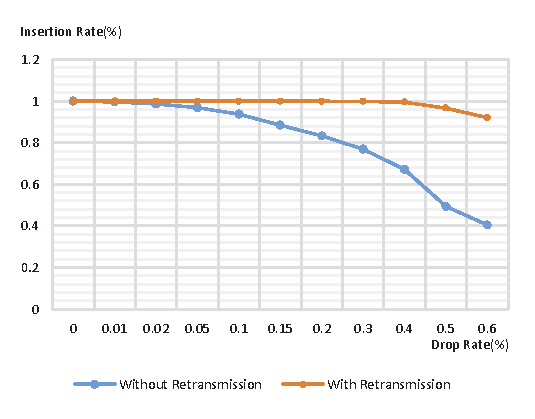
\includegraphics[width=0.7\textwidth]{drop-rate}
  \caption{不同丢包率情况下的数据插入成功率}
  \label{fig:drop-rate}
\end{figure}

\section{存储服务设计原则总结}
NDN Repo对外提供了远程的数据操作服务,并在Repo操作协议中定义了交换的文档格式,信息语义以及交互流程,具备了提供service的基本特征。根据web service的WSMF模型的八要素:Repo的协议已经具备如下要素:

\begin{itemize}
\item 文档类型(Document Types):确定协议间到底采用的是插入协议还是删除协议。
\item 语义(semantics):采用与NDN协议中相似的数据类型,例如:NAME-COMPONENT-TYPE。
\item 相关传输协议:采用NDN作为底层的传输协议。
\item 信息交换序列:完整的数据对象被底层NDN网络分段时,在分段数据包名字后加入了段序号。
\item 流程:无论是插入还是删除的协议都定义了相对完备的流程,在流程中出现的各种状态,都定义了repo的相应操作。
\item 安全:下层的NDN网络定义了针对数据包的基本安全,而在repo协议中对命令请求也进行了证书签名。
\item 句法:采用了TLV格式,同样具备动态伸缩的文档格式。此外由于在TLV格式中包含了数据的长度信息,文档编码解码的效率更高。
\item 服务配置:在repo-ng的实现过程中,repo-ng的配置文件采用了json格式,同时语义比较接近validconf。
\end{itemize}

由上可得,以NDN Repo协议为基础的NDN网络上的服务具备WSMF模型所要求的Web服务的基本要素,可以以repo协议为原型,提出一套基于命名数据网络的服务架构。而相比于Web Service的经典三要素:SOAP,UDDI以及WSDL,目前在基础设计上还是缺位的。具体体现在,虽然在Repo协议中定义了一些命令的消息格式,但是没有一套通用的命令格式。在NDN Packet Specification中,对TLV结构的格式有一套基本定义,但是还没有对命令及其参数等信息的文档描述。最后,在Web Service中UDDI为Web Service功能集成的典型目录系统,虽然NDN协议未必需要一个集成的服务目录,但是需要一套Service Descovery。进一步的为了服务流程自动化,NDN服务协议也需要一套类比于BPEL的服务集成方式。